
\documentclass[nooutcomes]{ximera}
%\documentclass[space,handout,nooutcomes]{ximera}

% For preamble materials

\graphicspath{
  {./}
  {algorithms/}
  {../algorithms/}
}


%%% This set of code is all of our user defined commands
\newcommand{\bysame}{\mbox{\rule{3em}{.4pt}}\,}
\newcommand{\N}{\mathbb N}
\newcommand{\C}{\mathbb C}
\newcommand{\W}{\mathbb W}
\newcommand{\Z}{\mathbb Z}
\newcommand{\Q}{\mathbb Q}
\newcommand{\R}{\mathbb R}
\newcommand{\A}{\mathbb A}
\newcommand{\D}{\mathcal D}
\newcommand{\F}{\mathcal F}
\newcommand{\ph}{\varphi}
\newcommand{\ep}{\varepsilon}
\newcommand{\aph}{\alpha}
\newcommand{\QM}{\begin{center}{\huge\textbf{?}}\end{center}}

\renewcommand{\le}{\leqslant}
\renewcommand{\ge}{\geqslant}
\renewcommand{\a}{\wedge}
\renewcommand{\v}{\vee}
\renewcommand{\l}{\ell}
\newcommand{\mat}{\mathsf}
\renewcommand{\vec}{\mathbf}
\renewcommand{\subset}{\subseteq}
\renewcommand{\supset}{\supseteq}
\renewcommand{\emptyset}{\varnothing}
\newcommand{\xto}{\xrightarrow}
\renewcommand{\qedsymbol}{$\blacksquare$}
\newcommand{\bibname}{References and Further Reading}
\renewcommand{\bar}{\protect\overline}
\renewcommand{\hat}{\protect\widehat}
\renewcommand{\tilde}{\widetilde}
\newcommand{\tri}{\triangle}
\newcommand{\minipad}{\vspace{1ex}}
\newcommand{\leftexp}[2]{{\vphantom{#2}}^{#1}{#2}}

%% More user defined commands
\renewcommand{\epsilon}{\varepsilon}
\renewcommand{\theta}{\vartheta} %% only for kmath
\renewcommand{\l}{\ell}
\renewcommand{\d}{\, d}
\newcommand{\ddx}{\frac{d}{dx}}
\newcommand{\dydx}{\frac{dy}{dx}}


\usepackage{bigstrut}


\newenvironment{sectionOutcomes}{}{}

\usepackage{array}
%\setlength{\extrarowheight}{-.2cm}   % Commented out by Findell to fix table headings.  Was this for typesetting division?  
\newdimen\digitwidth
\settowidth\digitwidth{9}
\def~{\hspace{\digitwidth}}
\def\divrule#1#2{
\noalign{\moveright#1\digitwidth
\vbox{\hrule width#2\digitwidth}}}


\title{Systematic Counting}
\author{Bart Snapp and Brad Findell and Jenny Sheldon}
\begin{document}
\begin{abstract}
Problems about systematic counting.
\end{abstract}
\maketitle


Easy counting problems are easy.  But in challenging counting problems, it becomes very important to use a systematic method for listing all of the possibilities.  Without a systematic approach, it is to easy to miss some possibilities or to    
list other possibilities more than once (or both). 

Here are some strategies that are very useful when solving such problems:  
\begin{itemize}
\item Fix one choice, and systematically change the other parts through all possibilities.  Change the first choice to the next option, and repeat.  
\item List the possibilities in dictionary or numerical order, either forward or backward. 
%\item Organize the possibilities into ``types,'' and then be systematic within each type.  
%\item Intentionally overcount, and then adjust systematically.  
\end{itemize}
These strategies can be combined.  And a ``road map'' can help you manage the process.     


Some examples are given below. 

\begin{problem}
A wedding planner offers three different entr\'ees (Beef, Chicken, and Vegetarian), four different sides (Fruit, Hummus, Pasta, and Salad), and two desserts (Ice cream and Tiramis\`u).  List all of the dinner possibilities.  

\begin{solution}
List them in dictionary order: 
\[
\begin{array}{c}
BFI \\
\answer[format=string]{BFT} \\
\answer[format=string]{BHI} \\
\answer[format=string]{BHT} \\
\answer[format=string]{BPI} \\
\answer[format=string]{BPT} \\
\answer[format=string]{BSI} \\
\answer[format=string]{BST} \\
CFI \\
\answer[format=string]{CFT} \\
\answer[format=string]{CHI} \\
\answer[format=string]{CHT} \\
\answer[format=string]{CPI} \\
\answer[format=string]{CPT} \\
\answer[format=string]{CSI} \\
\answer[format=string]{CST} \\
\answer[format=string]{VFI} \\
\answer[format=string]{VFT} \\
\answer[format=string]{VHI} \\
\answer[format=string]{VHT} \\
\answer[format=string]{VPI} \\
\answer[format=string]{VPT} \\
\answer[format=string]{VSI} \\
\answer[format=string]{VST} 
\end{array}
\]
Note that the entr\'ee is fixed first at \wordChoice{\choice[correct]{Beef} \choice{Chicken} \choice{Vegetarian}} with all of the possible side and dessert combinations, in dictionary order.  

Note also that the structure of this listing can help explain \textbf{why} there are 
$3\times\answer{4}\times\answer{2}=\answer{3\cdot 4\cdot 2}$ possible meals.  

Here is a road map that can help you imagine the above list as a process of systematically traveling all possible roads: 
\begin{center}
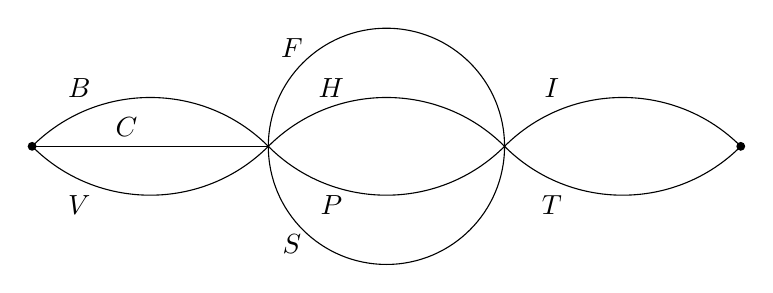
\begin{tikzpicture}
  \fill (0,0) circle (1.6pt);
%  \node [left] at (0,0) {$A$};
  \node [above] at (0.6,0.5) {$B$};
  \node [above] at (1.2,0) {$C$};
  \node [below] at  (0.6,-0.5) {$V$};
  \draw (0,0) to [out=45,in=135 ] (3,0);
  \draw (0,0) to (3,0);
  \draw (0,0) to [out=315,in=225] (3,0);
  \node [above] at (3.3,1.0) {$F$};
  \node [above] at (3.8,0.5) {$H$};
  \node [below] at  (3.8,-0.5) {$P$};
  \node [below] at  (3.3,-1.0) {$S$};
  \draw (3,0) to [out=45,in=135 ] (6,0);
  \draw (3,0) to [out=315,in=225] (6,0);
  \draw (4.5,0) circle (1.5);
  \node [above] at (6.6,0.5) {$I$};
  \node [below] at  (6.6,-0.5) {$T$};
  \draw (6,0) to [out=45,in=135 ] (9,0);
  \draw (6,0) to [out=315,in=225] (9,0);
  \fill (9,0) circle (1.6pt);
%  \node [right] at (8,0) {$B$};
\end{tikzpicture}
\end{center}


\end{solution}
\end{problem}


%\newpage 
%\begin{problem}
%List all of the factors of $5^3\cdot7^2\cdot11$. 
%
%\begin{solution}
% Choosing a factor is choosing the exponent of each of $5$, $7$, and $11$. 
% List the exponent triples in numerical order.  
%\[
%\begin{array}{c}
%5^0\cdot7^0\cdot11^0 \\
%5^0\cdot7^0\cdot11^1 \\
%5^0\cdot7^1\cdot11^0 \\
%\answer{5^0\cdot7^1\cdot11^1} \\
%\answer{5^0\cdot7^2\cdot11^0} \\
%\answer{5^0\cdot7^2\cdot11^1} \\ \\
%5^1\cdot7^0\cdot11^0 \\
%\answer{5^1\cdot7^0\cdot11^1} \\
%\answer{5^1\cdot7^1\cdot11^0} \\
%\answer{5^1\cdot7^1\cdot11^1} \\
%\answer{5^1\cdot7^2\cdot11^0} \\
%\answer{5^1\cdot7^2\cdot11^1} \\ \\
%5^2\cdot7^0\cdot11^0 \\
%\answer{5^2\cdot7^0\cdot11^1} \\
%\answer{5^2\cdot7^1\cdot11^0} \\
%\answer{5^2\cdot7^1\cdot11^1} \\
%\answer{5^2\cdot7^2\cdot11^0} \\
%\answer{5^2\cdot7^2\cdot11^1} \\ \\
%\answer{5^3\cdot7^0\cdot11^0} \\
%\answer{5^3\cdot7^0\cdot11^1} \\
%\answer{5^3\cdot7^1\cdot11^0} \\
%\answer{5^3\cdot7^1\cdot11^1} \\
%\answer{5^3\cdot7^2\cdot11^0} \\
%5^3\cdot7^2\cdot11^1
%\end{array}
%\]
%\end{solution}
%\end{problem}

\newpage
\begin{problem}
List all right-rectangular prisms of volume $24$ and whole-number sides.  Assume the three dimensions are distinguishable. 
\begin{solution}
\[
\begin{array}{|c|c|c|}
\hline
\text{length} & \text{width} & \text{height} \\ 
\hline
1 & 1 & 24 \\
1 & 2 & 12 \\
1 & 3 & 8 \\
1 & 4 & 6 \\
1 & 6 & 4 \\
1 & 8 & 3 \\
1 & 12 & 2 \\
1 & 24 & 1 \\
2 & 1 & 12 \\
2 & 2 & 6 \\
2 & 3 & 4 \\
2 & 4 & 3 \\
2 & 6 & 2 \\
2 & 12 & 1 \\
3 & 1 & 8 \\
3 & 2 & 4 \\
3 & 4 & 2 \\
3 & 8 & 1 \\
4 & 1 & 6 \\
4 & 2 & 3 \\
4 & 3 & 2 \\
4 & 6 & 1 \\
6 & 1 & 4 \\
6 & 2 & 2 \\
6 & 4 & 1 \\
8 & 1 & 3 \\
8 & 3 & 1 \\
12 & 1 & 2 \\
12 & 2 & 1 \\
24 & 1 & 1 \\
\hline
\end{array}
\]
In the solution, note that when the length has been fixed, the width and height are systematically varied in order of increasing $\answer[format=string]{width}$. Then, after all of the width-height combinations have been exhausted, the 
$\answer[format=string]{length}$ is changed to the next allowable value and ``refixed,'' and the width and height are again systematically varied.  
\end{solution}
\end{problem}

\newpage
\begin{problem}
Some readers may complain that the above list of volume-$24$ prisms contains much duplication.  And this would be true if we consider, for example, a $6\times4\times1$ prism to be the same as a $4\times1\times\answer{6}$ prism.  

Again, list all right-rectangular prisms of volume $24$ and whole-number sides.  This time, assume the three dimensions are \textbf{not} distinguishable. 

\begin{solution}
To prevent overcounting, require that 
$\text{length} \le \text{width} \le \text{height}$. 
\[
\begin{array}{|c|c|c|}
\hline
\text{length} & \text{width} & \text{height} \\ 
\hline
1 & 1 & 24 \\
\answer{1} & \answer{2} & \answer{12} \\
\answer{1} & \answer{3} & \answer{8} \\
\answer{1} & \answer{4} & \answer{6} \\
\answer{2} & \answer{2} & \answer{6} \\
\answer{2} & \answer{3} & \answer{4} \\
\hline
\end{array}
\]
How do we know we are done?  
\begin{freeResponse}
\begin{hint}
The next entry with a length of $2$ would be $(2,4,3)$, which is already listed---or which violates the condition that 
$\text{length} \le \text{width} \le \text{height}$.

The next length possibility would be $3$, and the first entry in such a row would be $(3,4,2)$, which is already listed. 
\end{hint}
\end{freeResponse}
\end{solution}
\end{problem}


\newpage
\begin{problem}
In the red/green light context, list all combinations of $2$ red lights from among $5$ lights.    
\begin{solution}
List in dictionary order: 
\[
\begin{array}{c}
GGGRR \\ \hline \\
\answer[format=string]{GGRGR} \\
\answer[format=string]{GGRRG} \\ \hline \\
\answer[format=string]{GRGGR} \\
\answer[format=string]{GRGRG} \\
\answer[format=string]{GRRGG} \\ \hline \\
\answer[format=string]{RGGGR} \\
\answer[format=string]{RGGRG} \\
\answer[format=string]{RGRGG} \\
\answer[format=string]{RRGGG}
\end{array}
\]
In the solution, note the separations demonstrating that once the position of the first red light is chosen, the $\answer[format=string]{second}$ red light systematically varies among all possible remaining positions, in dictionary order.  
\end{solution}
\end{problem}


\end{document}



